% Chapter Template

\chapter{Activity--Rotation--Age Investigation} % Main chapter title

\label{Chapter5} 

\epigraph{\itshape Sometimes the wheel turns slowly, but it turns.}{---Lorne Michaels}

\section{Introduction}

The results presented in Chapters \ref{Chapter3} and \ref{Chapter4} investigated the age-activity relationship through coronal and chromospheric emission. However, the age-activity relationship is a consequence of magnetic braking that removes angular momentum from the star on the main sequence. Thus, the age-activity relationship is inherently link to the rotational evolution. As discussed in Section \ref{Chp2_activity-rotation_lit_review}, this has led to studies on the activity-rotation relationship (see e.g. \citealt{Pizzolato_etal_2003,Wright_etal_2011}). The aim of this study was to collect literature values for the rotation period of the sample of stars considered in the two previous studies and investigate the activity-rotation relationship.

\subsection{Determining rotation periods}
\label{Chp5_Prot_methods}

There are several possible methods to determine the rotation period of a star; since the rotation periods considered in this work were collected from the literature and use various methods, they are summarised here for convenience.

The first method may be the most commonly used to determine the rotation period for a star - photometric variation in light curves due to starspots. As discussed in Section \ref{Chp1_photosphere}, starspots are observed in light curves as periodic variations in the brightness of star as the starspot rotates in and out of view of the observer. To obtain the stellar rotation period, techniques are used to detect periodicities in the light curve. One such technique is the Lomb-Scargle periodogram \citep{Lomb_1976,Scargle_1982}, which uses a Fourier transform to search for periodicities. Typically, a distribution of peaks will appear in the power spectrum and the period with the largest Lomb-Scargle power will correspond to the rotation period. It is a commonly used technique to determine the stellar rotation period (see e.g. \citealt{do_Nascimento_etal_2014,Nielsen_etal_2013}).

Another technique used to determine periodic variations in light curve is the autocorrelation function (ACF); this method determines how correlated the light curve is with itself when offset by a certain time lag. This can be performed for a range of time lags with repeated spot crossings providing peaks in the ACF at time periods associated with the rotation period. An advantage of this method is that the shape of the periodicity in the light curve is not assumed and thus may be more useful in cases where the modulation is not perfectly sinusoidal. This technique is also fairly common in the literature and has been used for large samples of stars from \textit{Kepler} \citep{McQuillan_etal_2014}.

The second method used to determine stellar rotation periods is long term observations of magnetic activity indicators such as the chromospheric emission from the \caII or \Halpha spectral lines and even X-ray luminosity. It is known that these magnetic activity indicators trace active magnetic regions on the surface, thus if an active region crosses the stellar surface multiple times then the rotation period can be determined from the modulation in the magnetic activity indicator. This technique is ideal for stars with more subtle light curve modulation (e.g. slower rotators) as magnetic activity indicators can trace smaller active regions. Examples of this method in the literature include \citet{Boro_Saikia_etal_2016,Robertson_etal_2015_GJ176,DeWarf_etal_2010}.

The third method that can be used to determine the rotation period is from asteroseismology. As discussed in Section \ref{Section:intro_ages}, asteroseismology is a valuable tool for determining fundamental parameters through observations of stellar oscillations. However, one aspect not discussed in the previous section is that any departure from solid body rotation will result in a frequency splitting of non-radial oscillation modes; thus the frequency will also depend on the azimuthal order, m. From helioseismology, the analysis of the frequency splitting due to rotation has provided detail about the interior of the Sun and revealed the presence of the tachocline \citep{Spiegel_Zahn_1992} which is instrumental in stellar dynamo theory . However, in order to obtain rotational splitting from asteroseismology, data sets with timescales on the order of years are required. This is due to the amplitude of the frequency splitting which vary from a few micro-Hertz for more massive or younger stars down to a fraction of a micro-Hertz for less massive or older stars. The frequency splitting of p modes in solar-like oscillators are predominantly determined by the rotational profile in the stellar envelope. There is still some debate in the literature about the accuracy of asteroseismic rotation periods (see e.g. \citealt{Barnes_etal_2016_aspect_gyro}), which will be discussed later in this Chapter.

\section{Data and Method}
\label{Chp5_data_and_method}

The sample of stars considered in this analysis comes from the X-ray luminosity and calcium emission studies conducted in Chapters \ref{Chapter3} and \ref{Chapter4}, respectively. Rotation periods for this sample of stars were searched for in the literature using \textit{VizieR} \citep{Ochsenbein_etal_2000}. In addition to this, literature values for the \Rprime activity indicator were collected for the sample of stars from the X-ray luminosity study. The details of the literature values collected and the relevant references for the sample of stars are shown in Appendix \ref{App_I_activity_rotation}.

Since the sample of stars considered in this work is fairly small, comparison samples from previous activity-rotation studies were also used. To compare the stars with values for the \Rprime indicator, the sample of stars from \citet{Metcalfe_etal_2016} were also plotted. Also, to put the asteroseismic samples into context, data was taken from \citet{Baliunas_etal_1996}. For the X-ray sample, data was taken from \citet{Wright_etal_2011} (W11) to put the sample into context.

As discussed in Section \ref{Chp2_activity-rotation_lit_review}, the activity-rotation relationship is usually calibrated in terms of Rossby number (\Ro). \Ro is defined as the as the rotation period divided by the convective turnover time (\tauc). In this work, \tauc was calculated using the relations from W11 that were derived empirically. By using an empirical method, it assumes that the activity-rotation relationship can be divided into saturated and non-saturated regimes. W11 divided their sample into bins of $B-V$ colour with approximately equal number of stars in each bin. For each mass bin, the activity-rotation relationship was fitted with Equation \ref{Eq:W11_tauc_method_fit_eq} where $(\frac{L_{x}}{L_{BOL}})_{sat}$ and $P_{sat}$ are fitted for each of the mass bins using the $\beta$ value found in W11.

\begin{equation}
    \frac{L_{x}}{L_{BOL}} = 
    \begin{cases}
        C_{B-V}P_{rot}^{\beta} & P_{rot} > P_{sat} \\
        (\frac{L_{x}}{L_{BOL}})_{sat} & P_{rot} < P_{sat}
    \end{cases}
    \label{Eq:W11_tauc_method_fit_eq}
\end{equation}

The fits from each mass bins were used by W11 to determine the colour dependent constant ($C_{B-V}$). The colour dependent constant is defined in Equation \ref{Eq:W11_tauc_method_CBV}, W11 found the colour dependence by setting the scaling constant (C) so that the \tauc value for solar-mass stars matched the values from \citet{Noyes_etal_1984}. This allowed for \tauc to be plotted as a function of colour and/or mass and the best-fitting relationship to be found. It is these best-fitting relationships shown in Equations \ref{Eq:W11_tauc_VK} and \ref{Eq:W11_tauc_mass} that are used to calculate \tauc in this work. In Equation \ref{Eq:W11_tauc_VK}, X is equal to $V-K$ and is valid in the range - $1.1 < V-K < 6.6$.

\begin{equation}
    C_{B-V} = C\tau_{c}^{-\beta}
    \label{Eq:W11_tauc_method_CBV}
\end{equation}

\begin{equation}
    \log \tau_{c} = 
    \begin{cases}
        0.73 + 0.22X & X < 3.5 \\
        -2.16 +1.50X - 0.13X^{2} & X > 3.5
    \end{cases}
    \label{Eq:W11_tauc_VK}
\end{equation}

\begin{equation}
    \log \tau = 1.16 - 1.49\log(M/M_{\odot}) - 0.54\log^{2}(M/M_{\odot})
    \label{Eq:W11_tauc_mass}
\end{equation}

For the majority of the samples considered in this analysis, masses were available and \tauc was calculated using Equation \ref{Eq:W11_tauc_mass}. However, for the sample of stars from \citet{Baliunas_etal_1996}, no masses were available. Therefore, Table 3 from \citet{Pecaut_etal_2012} was used to convert $B-V$ values into $V-K$ values and Equation \ref{Eq:W11_tauc_VK} was used to calculate \tauc. Since the table from \citet{Pecaut_etal_2012} is limited to $B-V < 0.77$, the sample from \citet{Baliunas_etal_1996} was also limited to stars that fell into this range.

\section{Results}

\subsection{Activity - rotation}
\label{Chp5_results_activity_rotation}

From the calcium emission study, eleven stars had rotation periods found in the literature; a further ten stars from the X-ray emission study had literature values for both the rotation period and the \Rprime activity indicator. In addition to this, data from \citet{Metcalfe_etal_2016} were used to compare and compliment the stars from the calcium and X-ray studies. Data from \citet{Baliunas_etal_1996} was also used to place the sample of old, slowly rotating stars with known ages into context.

Figure \ref{fig:rhk_v_rot} shows the \Rprime activity indicator as a function of rotation period for the sample of stars considered in this work. Stars from \citet{Baliunas_etal_1996}, \citet{Metcalfe_etal_2016} and my sample of stars are denoted by triangle, cross and circle symbols, respectively. Furthermore, the \citet{Metcalfe_etal_2016} data and the sample of stars considered in this work are presented by spectral type; F-type stars are shown in blue, G-type stars in green, K-type stars in orange and M-type stars in red. Figure \ref{fig:rhk_v_rot} shows that, as expected, there is a fair amount of scatter in the rotation period for a given activity level. Calculating the Pearson coefficient for the \citet{Baliunas_etal_1996} sample gives a value of $-0.59$, indicating that there is a negative correlation between the two parameters but they are not perfectly anti-correlated. The sample of stars from this work and \citet{Metcalfe_etal_2016} also follow a similar trend and generally agree with the \citet{Baliunas_etal_1996} sample. The exception to this is the M-type stars that have extremely long rotation periods, which is to be expected since they stay on the main sequence for much longer than F, G or K stars and therefore have much longer spin-down timescales.

\begin{figure}
    \centering
    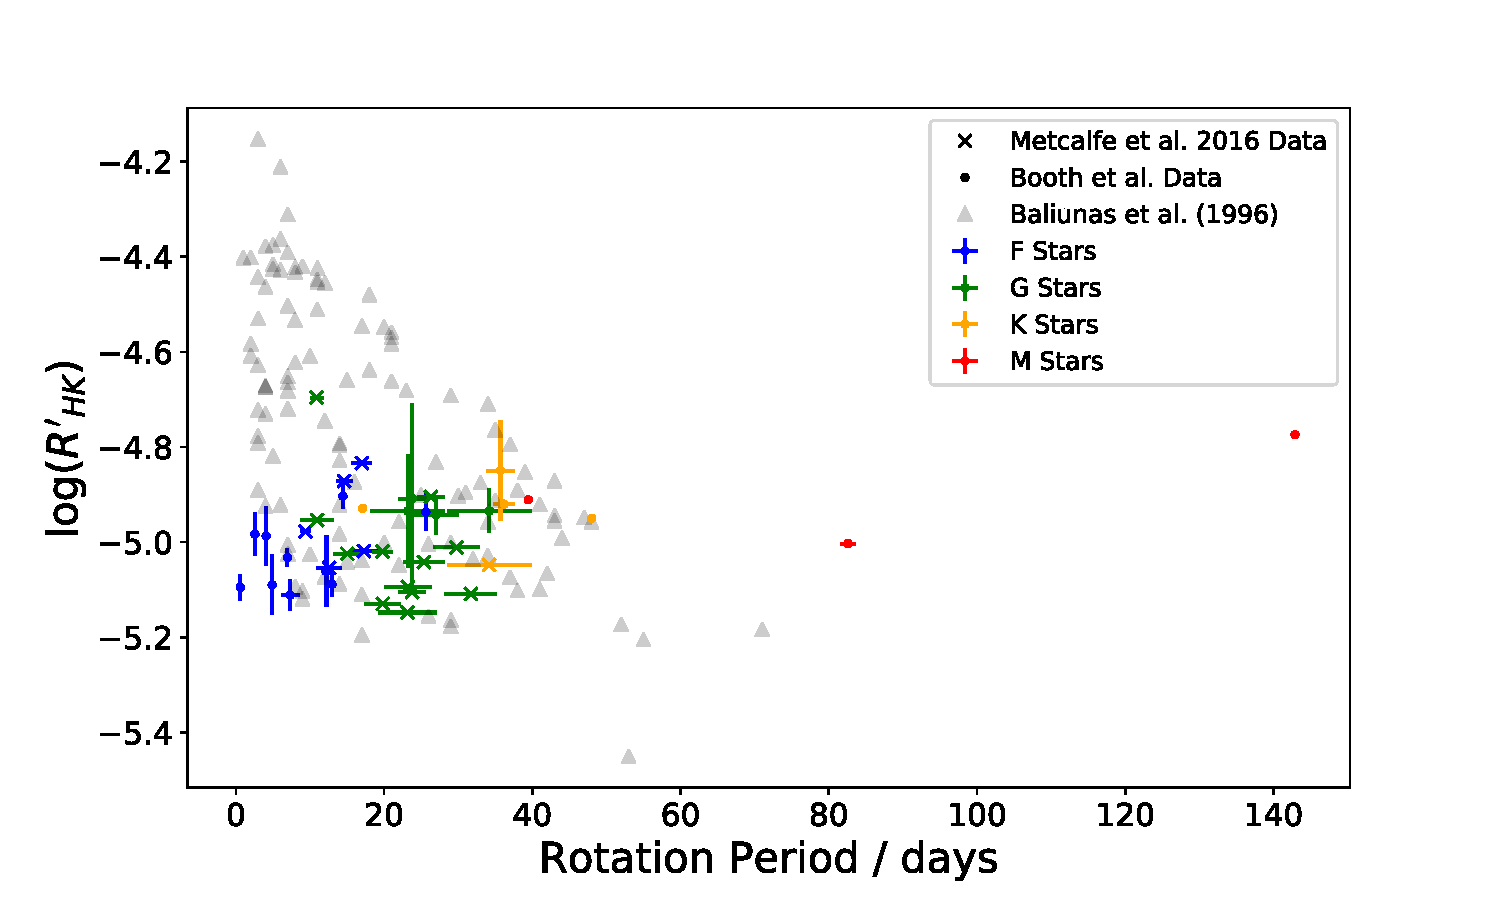
\includegraphics[width=0.95\textwidth]{Figures/5-Activity_rotation/Rhk_v_prot.pdf}
    \caption[\Rprime indicator as a function of rotation period]{Plot of the \Rprime indicator as a function of rotation period. Stars from \citet{Metcalfe_etal_2016} and this work are divided into the relevant spectral type.}
    \label{fig:rhk_v_rot}
\end{figure}

In line with previous activity-rotation studies \citep{Mamajek_Hillenbrand_2008,Metcalfe_etal_2016} we consider the Rossby number instead of rotation period, as shown in Figure \ref{fig:rhk_v_ro}. Note that in order to calculate \Ro for the \citet{Baliunas_etal_1996} sample, the sample was limited to $B-V < 0.77$ as discussed in Section \ref{Chp5_data_and_method}. As expected, the Pearson coefficient value of $-0.66$ shows a stronger negative correlation between the \Rprime indicator and \Ro for the limited \citet{Baliunas_etal_1996} sample of stars. Despite the use of \Ro, there is still a significant spread in \Ro for a given activity level, particularly for low activity levels. Figure \ref{fig:rhk_v_ro} also shows the activity-rotation relationship from \citet{Mamajek_Hillenbrand_2008} (MH08) for comparison, this relationship is valid in the range $-5.0 < \log(R^{'}_{HK}) < -4.3$. The MH08 activity-rotation relationship seems to describe the high activity level for a given Rossby number fairly well. However, there are many lower activity stars that cannot be accurately described by the MH08 relationship. There could be several reasons for this; one possibility is that the MH08 relationship is biased towards more active stars that have detectable light curve modulation due to starspots. Alternatively, as discussed in Section \ref{Chp4_discussion}, the stellar metallicity has an effect on the value of the \Rprime indicator calculated therefore it could be possible that some of this scatter in \Ro for a given activity level is due to metallicity effects.

\begin{figure}
    \centering
    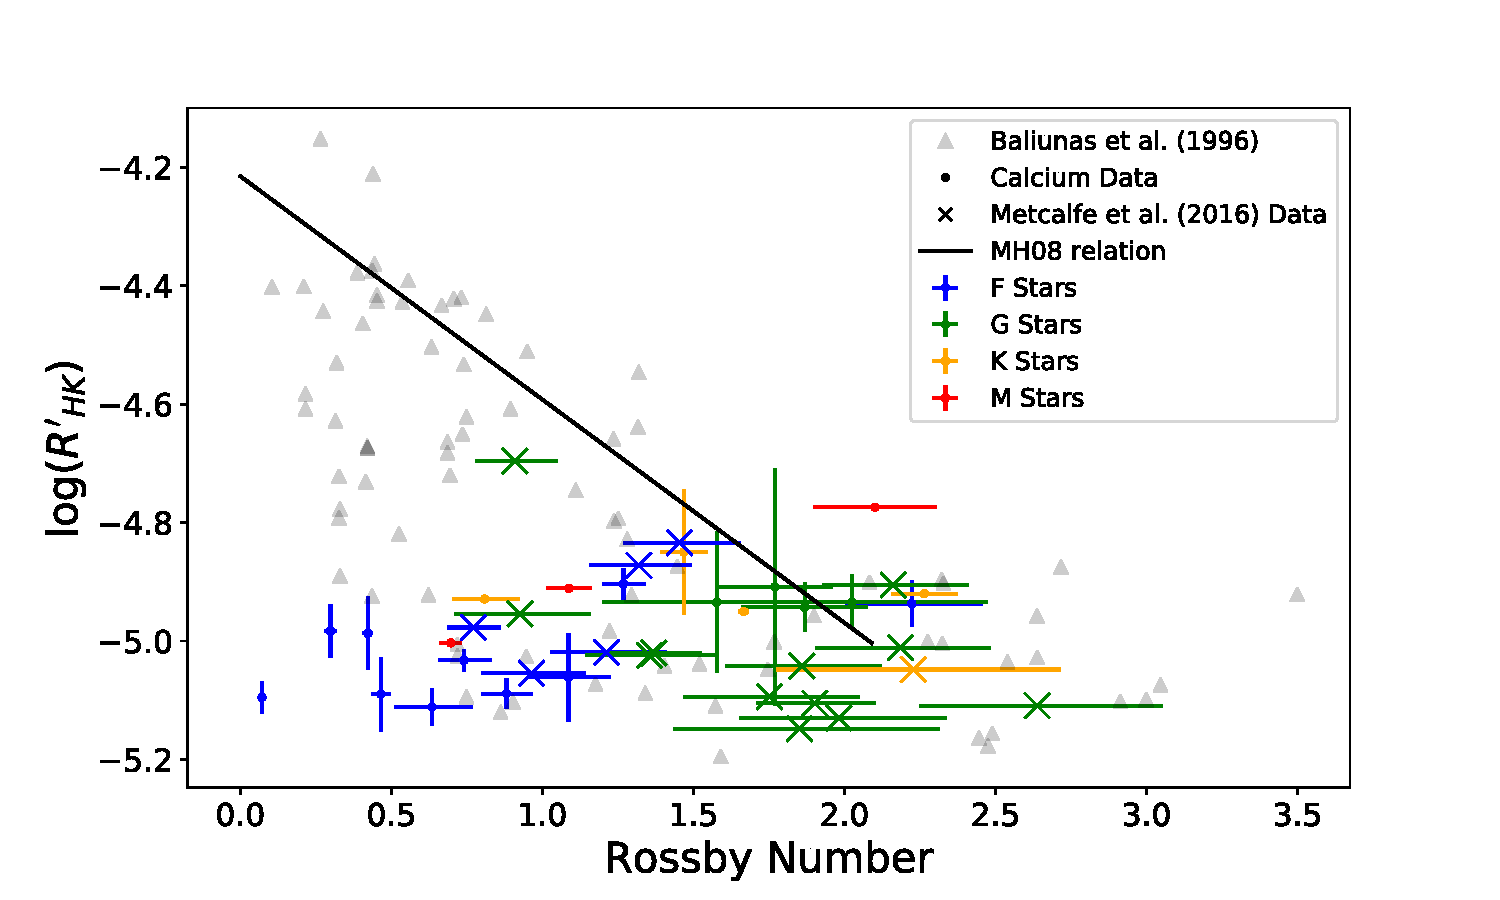
\includegraphics[width=0.95\textwidth]{Figures/5-Activity_rotation/rhk_v_r0.pdf}
    \caption[\Rprime indicator as a function of \Ro]{Plot of the \Rprime indicator as a function of \Ro. The activity-rotation relationship from \citet{Mamajek_Hillenbrand_2008} is shown in black for reference.}
    \label{fig:rhk_v_ro}
\end{figure}

%There are several stars considered in this work that are also present in the \citet{Metcalfe_etal_2016} sample, these are KIC 9139151, KIC 9955598, KIC 10454113 and KIC 10963065. Table \ref{tab:duplicate_stars_m16_diff} shows the absolute differences in their activity and rotation measurements from the sources used in this work and the values presented in \citet{Metcalfe_etal_2016}. Generally, there is good agreement between the activity and rotation parameters used in the two studies.

% \begin{table}[]
%     \centering
%     \renewcommand{\arraystretch}{1.2}
%     \begin{tabular}{lcc}
%         \hline
%         Star & $|\Delta\log R^{'}_{HK}|$ & $|\Delta P_{rot}|$ / days \\
%         \hline
%         KIC 9139151 & 0.107 & 1.260 \\
%         KIC 9955598 & 0.114 & 0.00 \\
%         KIC 10454113 & 0.031 & 0.162 \\
%         KIC 10963065 & 0.035 & 0.380 \\
%         \hline
%     \end{tabular}
%     \caption{Stars that are present in both the sample considered in this work and in \citet{Metcalfe_etal_2016}. The absolute value of the differences in the activity and rotation parameters are shown.}
%     \label{tab:duplicate_stars_m16_diff}
% \end{table}

Twelve stars from the X-ray study \citep{Booth_etal_2017} with determined X-ray luminosities (i.e. not upper limit results) were found to have rotation periods in the literature. This stellar sample is plotted as a function of \Ro alongside the W11 sample of stars as shown in Figure \ref{fig:lx_v_ro}. This plot shows that the sample of old, inactive stars generally lie in the unsaturated regime of the activity-rotation relationship, as expected. However, our sample tends to lie on the lower activity end of the scatter in the activity-rotation relationship. \textcolor{red}{Insert here that more in agreement with beta=-2.7 slope if I put that relationships in Fig 5.3}. The inclusion of the old, inactive sample of stars cannot confirm the potential steepening of the activity-rotation relationship as suggested by \citet{Booth_etal_2017}.

\begin{figure}
    \centering
    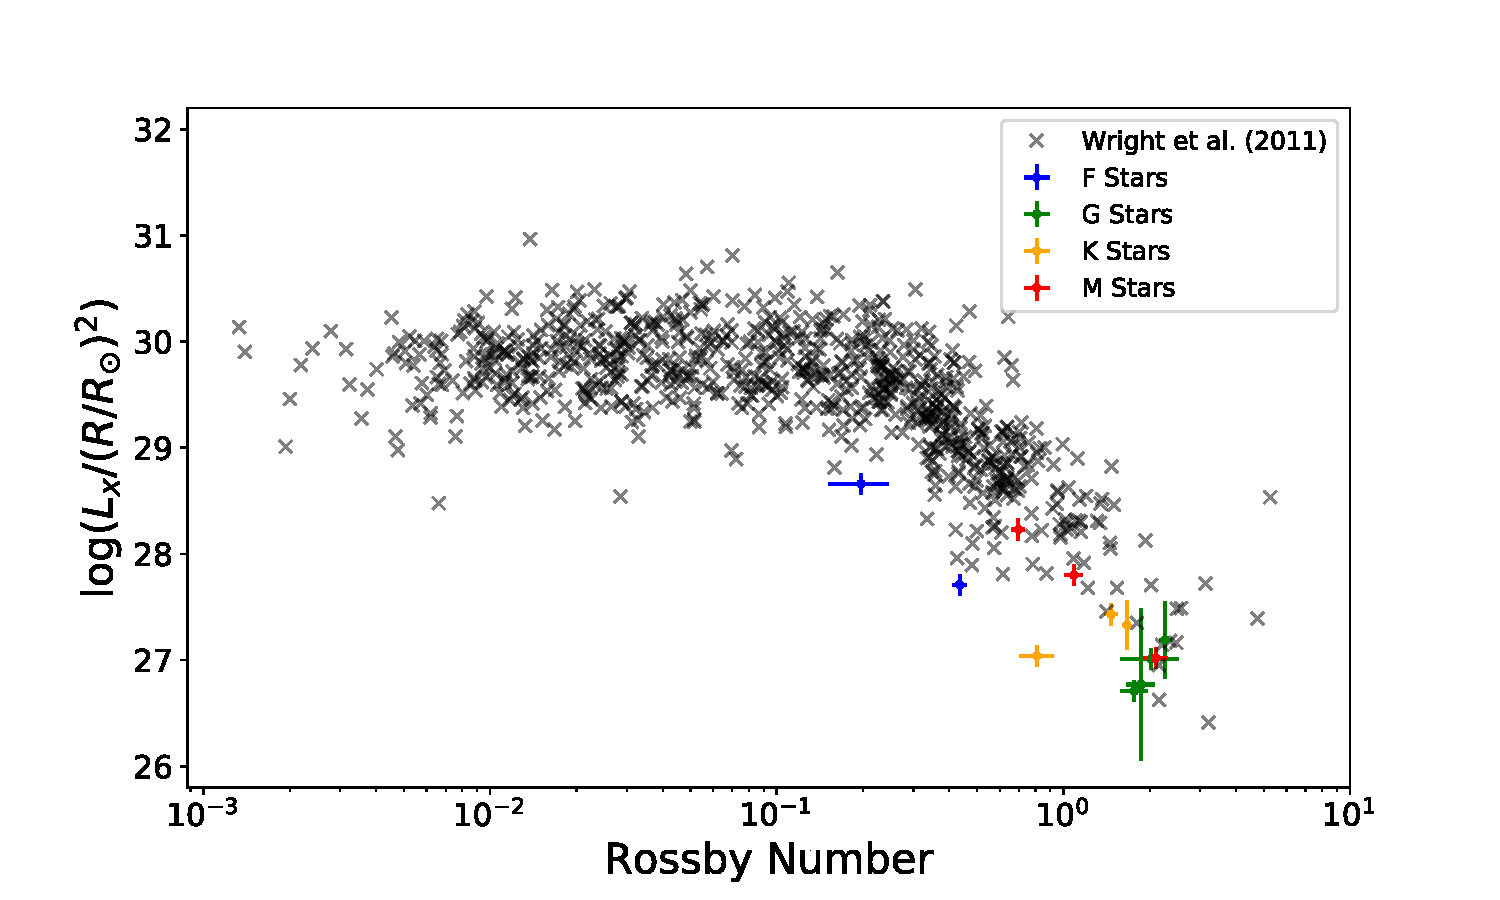
\includegraphics[width=0.95\textwidth]{Figures/5-Activity_rotation/lx_v_R0.pdf}
    \caption[$L_{x}$ as a function of \Ro]{X-ray luminosity normalised by stellar surface area as a function of \Ro for the sample of stars from the X-ray study with literature rotation periods. The sample from \citet{Wright_etal_2011} is plotted for comparison.}
    \label{fig:lx_v_ro}
\end{figure}

\subsection{Rotation--age}
\label{Chp5_results_rotation_age}
The collection of literature rotation periods for the sample of stars from the X-ray and calcium emission studies also gives the opportunity to investigate the rotation--age relationship. In total, 29 stars from the calcium and X-ray studies have literature rotation periods that are shown in Figure \ref{fig:full_sample_prot_v_age} alongside additional data from \citet{Metcalfe_etal_2016}. Since stellar spin-down is inherently dependent on the mass of the star, the sample was divided into the relevant spectral types for further investigation. 

\begin{figure}
    \centering
    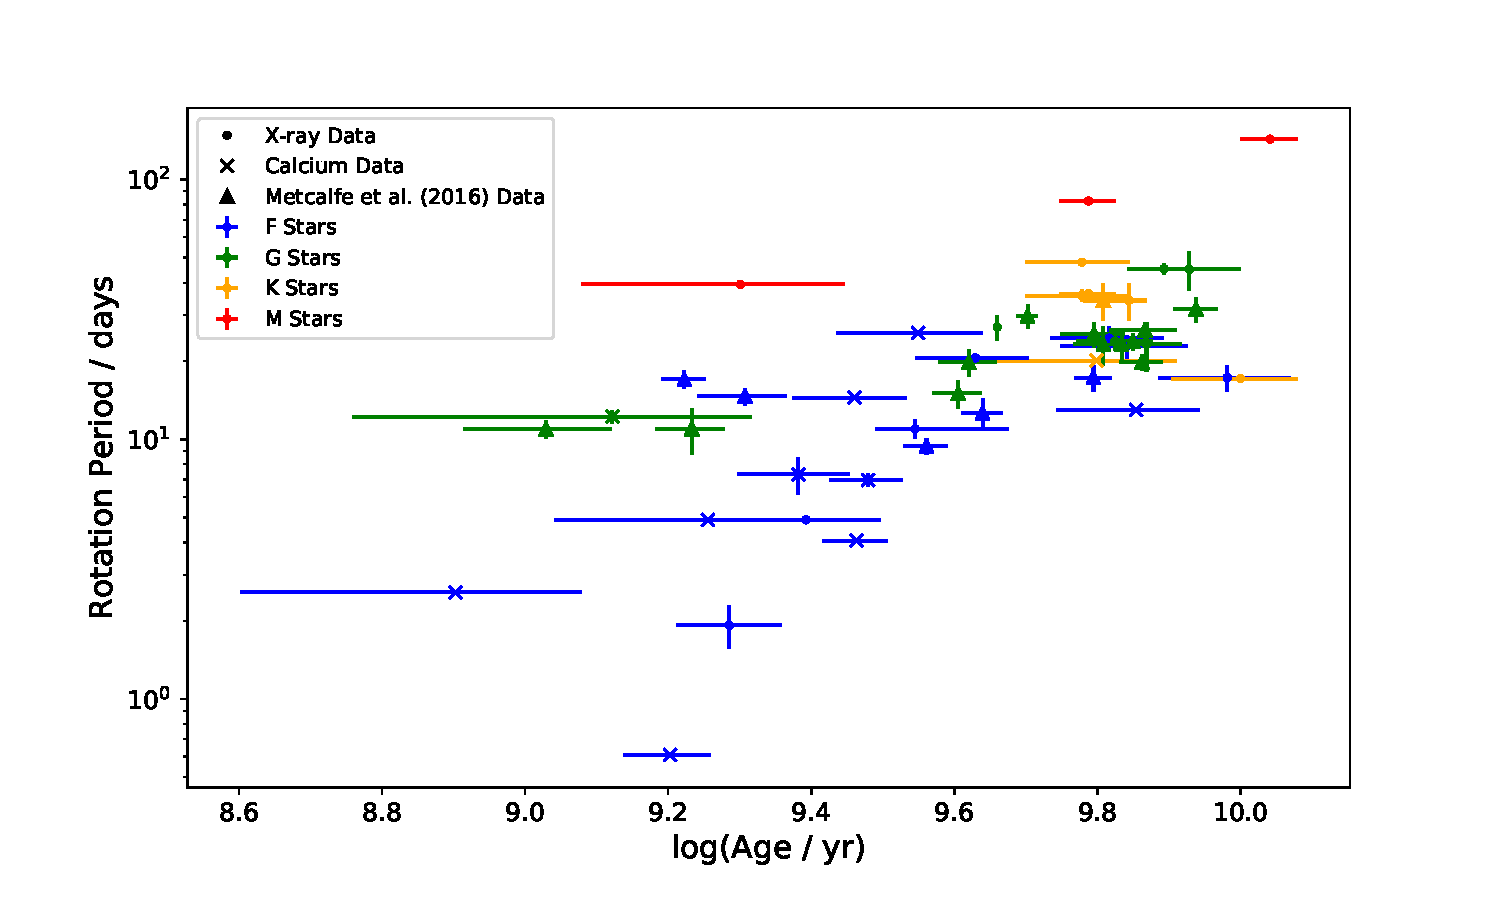
\includegraphics[width=0.95\textwidth]{Figures/5-Activity_rotation/prot_v_age.pdf}
    \caption{Logarithmic plot of rotation period as a function of age for our sample of stars alongside additional data from \citet{Metcalfe_etal_2016}. Stars are displayed by spectral type with the marker denoting the source of the data.}
    \label{fig:full_sample_prot_v_age}
\end{figure}

For each spectral type sample, an ODR was performed on the data using symmetric errors in age and $\log(P_{rot})$ to find the best--fitting relationship between rotation and age. This best--fitting relationship is plotted in black in Figures REF. The \citet{Barnes_2007} gyrochronology relationship was also used for comparison to the sample of old stars. The \citet{Barnes_2007} relationship was calculated for the mean B-V colour of the spectral type sample and plotted in red in Figures REF. It should be noted that the \citet{Barnes_2007} relationship has an age exponent of 0.52, similar to the Skumanich Law. In order to put the sample of old, inactive stars into context, data for clusters were obtained from the literature. These clusters are M67 and Praesepe with rotation periods taken from \citet{Barnes_etal_2016} and \citet{Douglas_etal_2017}, respectively. The ages of M67 and Praesepe are taken to be 4~Gyr and 650~Myr, respectively.

Figure \ref{fig:f_prot_v_age} shows the F-type stars in the sample along with the cluster data and the \citet{Barnes_2007} relationship. Due to the small errors associated with the rotation periods of the F-type stars and the relatively large errors in age, the ODR found a best-fitting relationship that had large uncertainties in both the gradient and y--intercept. Therefore, for this sample of stars, a linear regression was used. The best fitting relationship from the linear regression is shown in green in Figure \ref{fig:f_prot_v_age}. While the linear regression fit does not take into account the errors associated with the parameters, it gives a much more reasonable best--fitting relationship than the ODR method for this particular sample of stars. The best--fitting relationship for the F stars is shown in Equation \ref{Eq:f_stars_lin_reg} where $t$ is the stellar age in years.

\begin{equation}
    \log(P_{rot}) = (0.91 \pm 0.33)\log(t) -7.69
    \label{Eq:f_stars_lin_reg}
\end{equation}

\begin{figure}
    \centering
    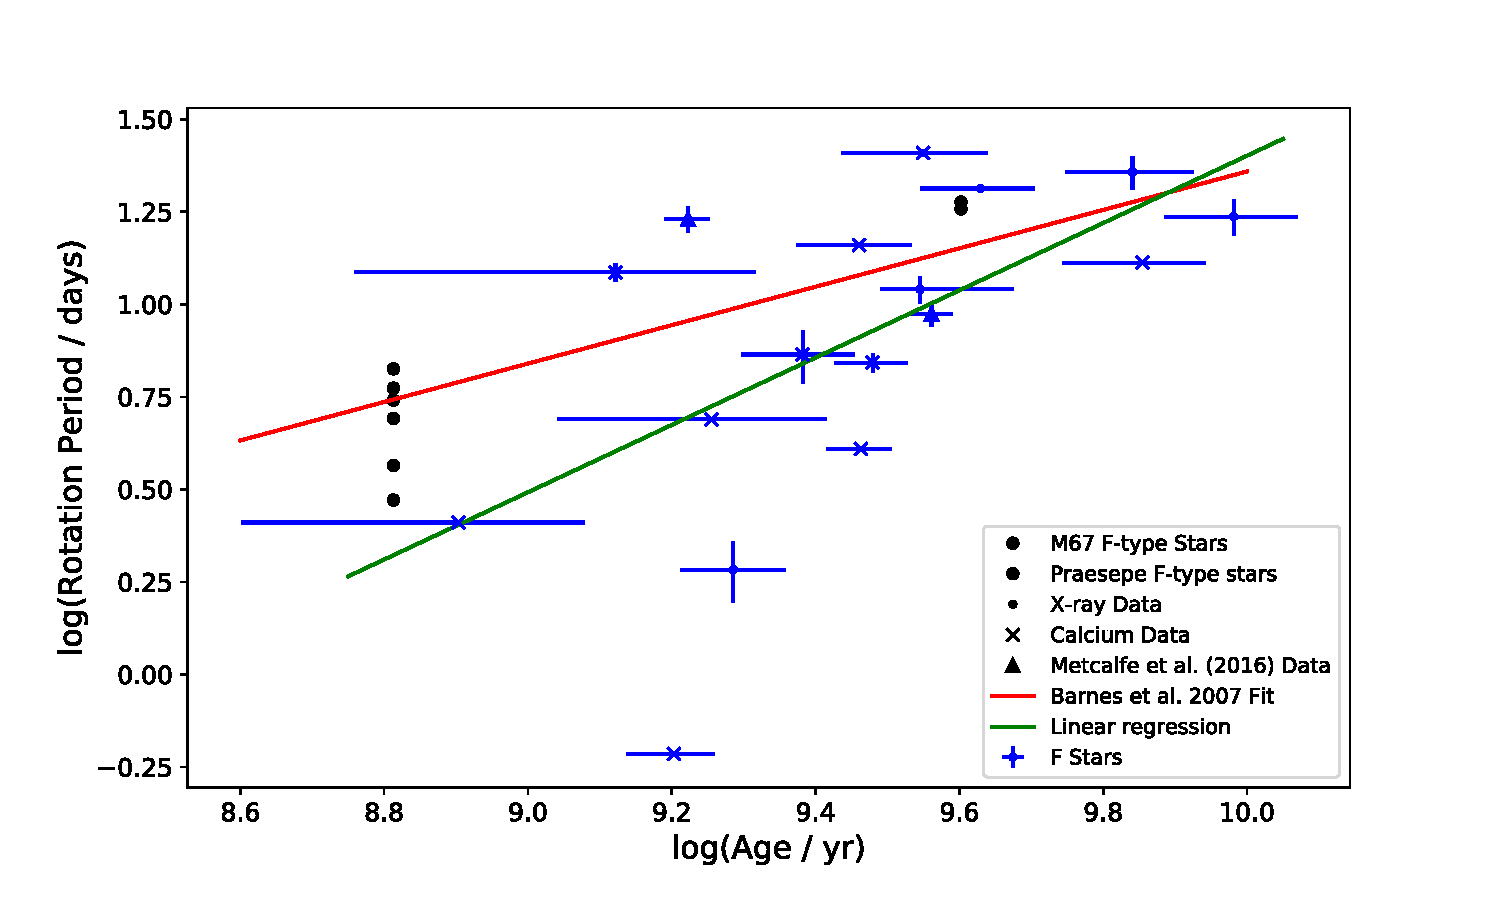
\includegraphics[width=0.95\textwidth]{Figures/5-Activity_rotation/f_prot_v_age_LR.pdf}
    \caption{Sample of F-type stars with the best--fitting relationship from linear regression shown in green and the \citet{Barnes_2007} gyrochronology relationship for the mean $B-V$ colour of the sample shown in red. Cluster data from M67 and Praesepe are also shown for comparison.}
    \label{fig:f_prot_v_age}
\end{figure}

Figure \ref{fig:f_prot_v_age} shows that the linear regression best--fitting relationship is steeper than the gyrochronology relationship. The gyrochronology relationship seems to be a reasonable fit for the slower rotators in the sample of F-type stars but not the young, fast rotators in the sample. However, the cluster data is in agreement with the \citet{Barnes_2007} relationship and rotate much slower than the best-fitting relationship found in this work would predict.

Figure \ref{fig:g_prot_v_age} shows the sample of G-type stars along with the cluster data, the \citet{Barnes_2007} relationship and the ODR best-fitting relationship. The best-fitting relationship as found by the ODR method is shown in Equation \ref{Eq:g_stars_ODR}. Similarly to the F-type stars, the gyrochronology relationship agrees with the cluster data and the slower rotators in the sample while the best-fitting relationship does not agree with the cluster data.


\begin{equation}
    \log(P_{rot}) = (0.86 \pm 0.19)\log(t) - (7.00 \pm 1.84)
    \label{Eq:g_stars_ODR}
\end{equation}

\begin{figure}
    \centering
    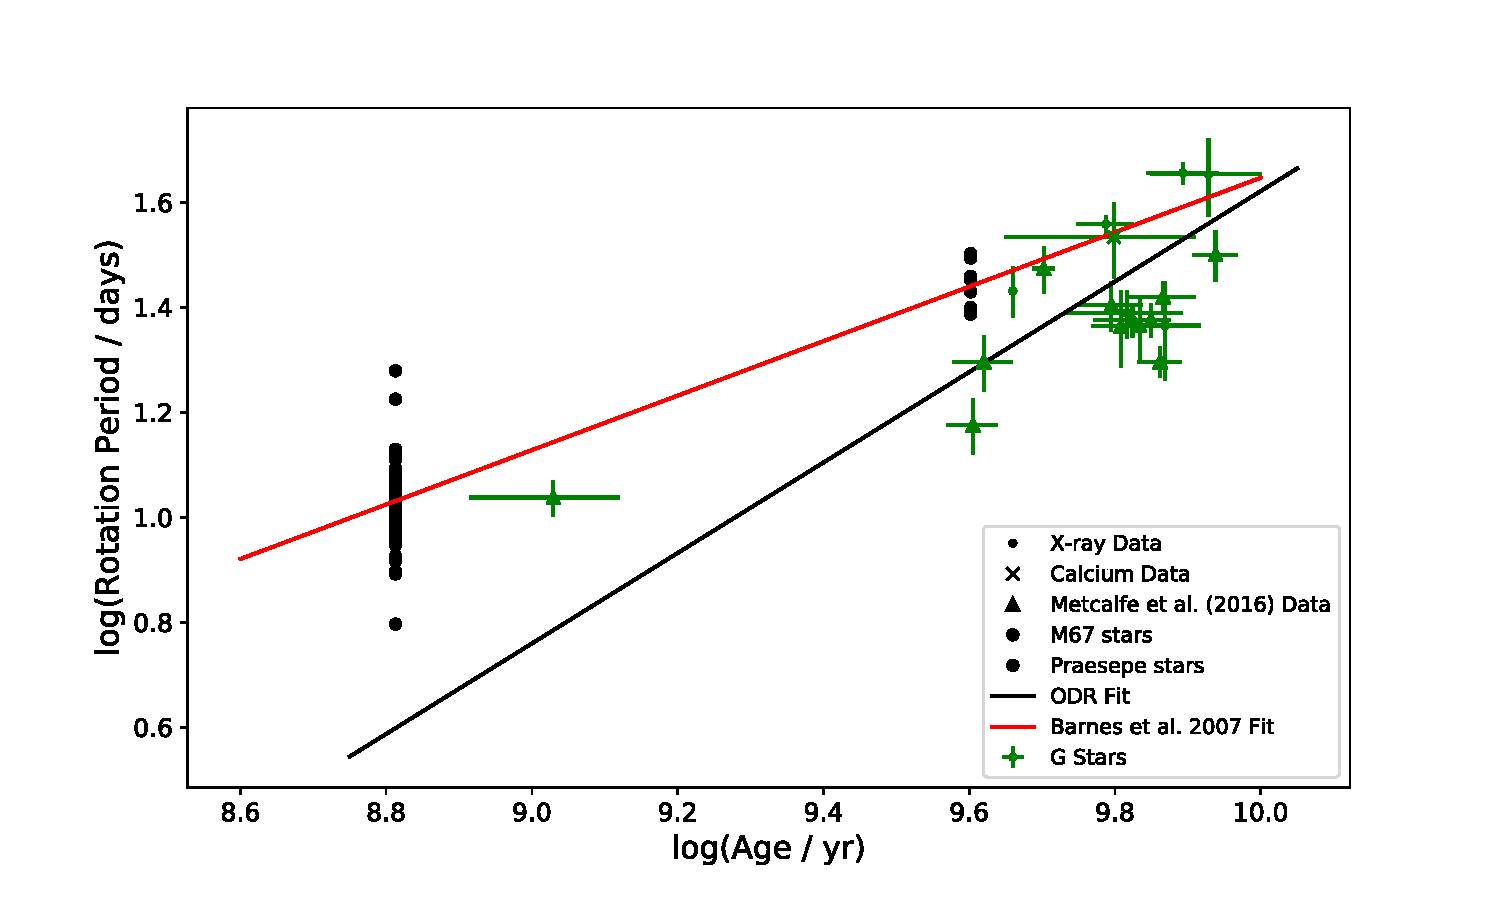
\includegraphics[width=0.95\textwidth]{Figures/5-Activity_rotation/g_prot_v_age.pdf}
    \caption{Sample of G-type stars with the best--fitting relationship from ODR shown in black and the \citet{Barnes_2007} gyrochronology relationship for the mean $B-V$ colour of the sample shown in red. Cluster data from M67 and Praesepe are also shown for comparison.}
    \label{fig:g_prot_v_age}
\end{figure}

Figure \ref{fig:k_prot_v_age} shows the sample of K-type stars along with the cluster data and the \citet{Barnes_2007} relationship. Only three stars in the sample are K dwarfs and are sufficiently diverse in age to accurately perform an ODR fit. It is interesting to note that the M67 K-type stars seem to lie below the gyrochronology relationship, this could be due to the difficulty of retrieving longer rotation periods from \textit{K2} data as discussed by \citet{Esselstein_etal_2018}.

\begin{figure}
    \centering
    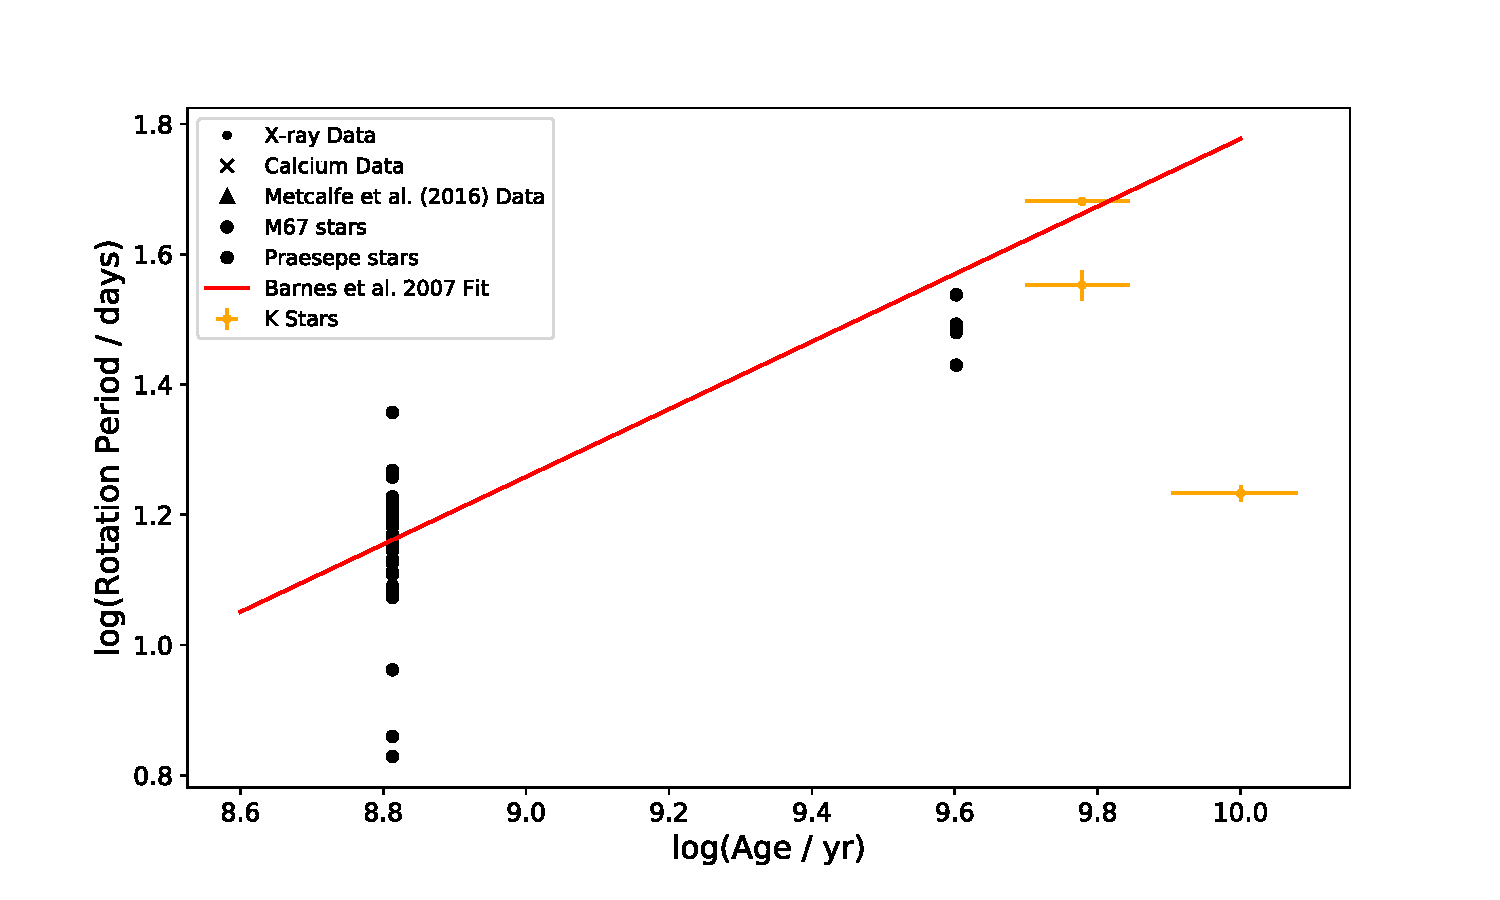
\includegraphics[width=0.95\textwidth]{Figures/5-Activity_rotation/k_prot_v_age.pdf}
    \caption{Sample of K-type stars with the \citet{Barnes_2007} gyrochronology relationship for the mean $B-V$ colour of the sample shown in red. Cluster data from M67 and Praesepe are also shown for comparison.}
    \label{fig:k_prot_v_age}
\end{figure}

\begin{figure}
    \centering
    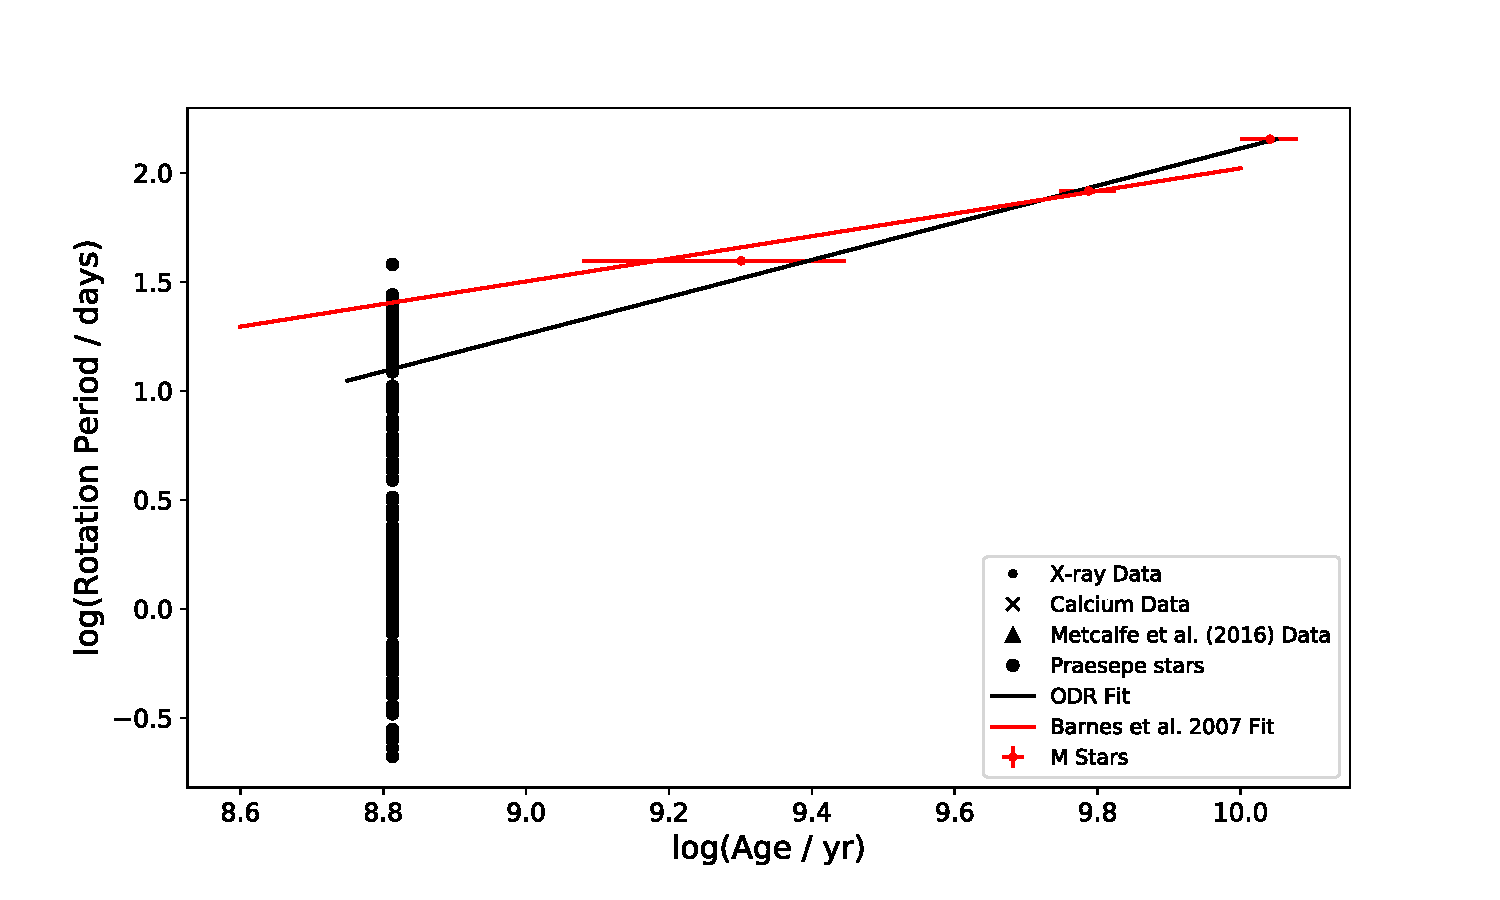
\includegraphics[width=0.95\textwidth]{Figures/5-Activity_rotation/m_prot_v_age.pdf}
    \caption{Sample of M-type stars with the best--fitting relationship from ODR shown in black and the \citet{Barnes_2007} gyrochronology relationship for the mean $B-V$ colour of the sample shown in red. Cluster data from M67 and Praesepe are also shown for comparison.}
    \label{fig:m_prot_v_age}
\end{figure}

Lastly, Figure \ref{fig:m_prot_v_age} shows the M-type stars along with the cluster data from the Praesepe cluster, the \citet{Barnes_2007} relationship and the ODR best-fitting relationship. The best-fitting relationship as found by the ODR method is shown in Equation \ref{Eq:m_stars_ODR}. Note that since the M dwarf stellar sample consits of only three data points, the ODR fit may not be representative of a larger stellar sample. The Praesepe cluster data from \citet{Douglas_etal_2017} was focused on low-mass stars, hence the large number of data points from the cluster in Figure \ref{fig:m_prot_v_age}. The M-type stars in Praesepe also have a large range of rotation periods which is not surprising given that M-type stars take the longest time to converge onto the 'I' sequence to use the terminology from \citet{Barnes_2003}. One may also question the validity of the gyrochronology relationship at these low masses. The \citet{Barnes_2007} relationship was calibrated to a $B-V \approx 1.6$ and the average $B-V$ value of the M-type stars in the sample is $1.65$. Therefore, the gyrochronology may not be accurate in this regime.

\begin{equation}
    \log(P_{rot}) = (0.85 \pm 0.11)\log(t) - (6.41 \pm 1.04)
    \label{Eq:m_stars_ODR}
\end{equation}



\section{Discussion}

\subsection{Rotation--age relationship}
The rotation--age relationships presented in Section \ref{Chp5_results_rotation_age} show that the best--fitting relationships found for the sample of old, inactive stars are not in agreement with the the slower rotators in the sample or the cluster data. However, the \citet{Barnes_2007} relationship is generally in agreement with the cluster data and the slower rotators in the sample. This result could be interpreted in two different ways, either the data suggests that older stars spin faster than expected similar to the conclusion made by \citet{van_Saders_etal_2016} or that the rotation periods collected are biased towards to faster stellar rotators.

The conclusion that the stellar sample are biased towards faster rotators is a valid concern especially considering that the rotation periods for the majority of the sample stem from light curve modulation caused by starspots. This method in particular is biased towards short rotation periods as it requires a detectable signal caused by fairly large starspots. As stars age and start to spin down, longer timescales are needed to detect variability due to starspots. In addition to this, older stars have fewer and smaller starspots \textcolor{red}{REF?} making measurement of the rotation period via this method even more difficult.

To test the hypothesis that older stellar samples are biased towards faster rotators, alternative methods of determining the stellar rotation period are needed. One alternative method is the long-term monitoring of magnetic activity indicators such as the \Rprime indicator. Since the \Rprime indicator traces areas of magnetic activity such as plage \citep{Leighton_1959}, precise calculation of this indicator coupled to observations over several rotation periods can yield the rotation period. This method has been used to determine the rotation for several of the stars considered in this work, particularly for stars that have longer rotation periods \citep{Boro_Saikia_etal_2016,Vaughan_etal_1981,Robertson_etal_2015_GJ191}. This method requires a number of observations over the timescale of several rotation periods to ensure that the \Rprime indicator is sampled sufficiently to accurately determine the rotation period. However, this method also has the advantage of gaining information about the variability of the magnetic activity over a longer timescale.

An alternative method for determining the stellar rotation period is from asteroseismology. Departures from solid body rotation result in frequency splitting of non-radial oscillation modes and thus the frequency is also dependent on the azimuthal order, m. As discussed in Section \ref{Chp5_Prot_methods}, the frequency splitting of p modes observed in main--sequence stars are largely determined by the rotation profile in the stellar envelope. This is an important aspect of this method, if the stellar rotation period determined from asteroseismology is not the stellar surface rotation, can it be used in gyrochronology relationships? It is this question that makes asteroseismic rotation periods controversial \citep{Barnes_etal_2016_aspect_gyro}. However, some asteroseismology studies find good agreement between the rotation periods determined from asteroseismology and other surface rotation measures \citep{Chaplin_etal_2013,Gizon_etal_2013}. This includes \citet{Davies_etal_2015} who determined the rotation periods for 16 Cyg A \& B from asteroseismology. As an independent validation, they also performed the same analysis on solar data by adding white noise comparable to that found for the stellar data. They find that the asteroseismic rotation for the Sun to be $28.2^{+0.9}_{-1.0}$~days which is consistent with the Carrington rotation period of $27.28$~days. \citet{Davies_etal_2015} suggest that the agreement may be because of an absence of significant differential rotation. They conclude that for 16 Cyg A, the asteroseismic rotation is comparable to surface rotation on the assumption that there is an absence of strong radial differential rotation. Therefore, care needs to be taken when considering asteroseismic rotation periods.

\subsection{Activity-rotation relationship}
In Section \ref{Chp5_results_activity_rotation}, the literature rotation periods were used to investigate the activity--rotation relationship for the sample of old, inactive stars. Two activity indicators, calcium and X-ray emission, were considered and here I will discuss the results in the context of recent observational and theoretical studies.

The \Rprime activity indicator was plotted as a function of Rossby number in Figure \ref{fig:rhk_v_ro}. This plot shows that there is significant scatter in the \Rprime--\Ro relationship, this is partly due to mass since this will influence the timescale of the stellar spin-down. However, as discussed in Chapter \ref{Chapter4}, metallicity has a significant effect on the value of the \Rprime activity indicator. This may explain why the activity-rotation from \citet{Mamajek_Hillenbrand_2008} does not fully describe the full sample of old stars or the sample from \citet{Baliunas_etal_1996}.

Figure \ref{fig:lx_v_ro} showed the X-ray luminosity as a function of Rossby number, this clearly showed that the old sample of stars is in general agreement with the previous study by \citet{Wright_etal_2011}. \textcolor{red}{The old sample of stars may be more in favour for a slope of -2.7 for the activity-rotation relationship as \citet{Wright_etal_2011} found for a small, unbiased sample of their data. -- Confirm this once I put slopes in Fig 5.3.} While the old sample of stars considered in this work may give more evidence towards a slight steepening of the activity--rotation relationship, this amount of change in the slope would not be sufficient by itself to warrant the steepening of the X-ray luminosity--age relationship presented in Chapter \ref{Chapter3}. In addition to this, with the report of weakened magnetic braking for older stars \citep{van_Saders_etal_2016}, the slope of the activity--rotation relationship would have to increase further to explain the result in Chapter \ref{Chapter3}. 

This result would indicate that an alternative method is responsible for the steepening of the age--activity relationship. One possible 


























\section{Conclusions}


























